\section{Problem and Environment}

\textbf{Motivation.} Platelets have a maximum shelf life of only 3--5 days after testing~\cite{abouee2023platelet}, and daily usage is highly variable~\cite{motamedi2021platelet}. A blood bank that orders too much throws away expired units, and one that orders too little must place emergency orders or delay transfusions. Every day the bank has to decide how many units of each of the 8 ABO/Rh groups to order, so this is a sequential decision problem under uncertainty, which we formulate as a Markov decision process (MDP) and solve with reinforcement learning.

\textbf{Demand calibration.} Hospital transfusion records are private clinical data, so no public daily demand dataset exists. We therefore simulate demand and calibrate it to published statistics. Daily demand of each group is negative binomial, with variance/mean ratio $12.3/5.4 \approx 2.28$ as observed in a network of Canadian hospitals, where demand was found to be overdispersed and was also fitted with a negative binomial per weekday~\cite{abouee2023platelet}. The weekday pattern of the mean total demand (Mon--Sun: 28.8, 33.4, 26.2, 28.4, 30.8, 18.6, 19.6 units) is taken from University College London Hospitals data~\cite{uclh2024platelet}. Total demand is split over groups using shares that approximate the Indian donor population (O 37\%, B 32\%, A 23\%, AB 8\%, about 5\% Rh negative~\cite{indiabloodgroups}); we use O+/O$-$ 33/2.5\%, B+/B$-$ 31/2\%, A+/A$-$ 21/1.5\% and AB+/AB$-$ 8/1\%. Fig.~\ref{fig:demand} shows that the simulator reproduces the target weekday means.

\begin{figure}[t]
  \centering
  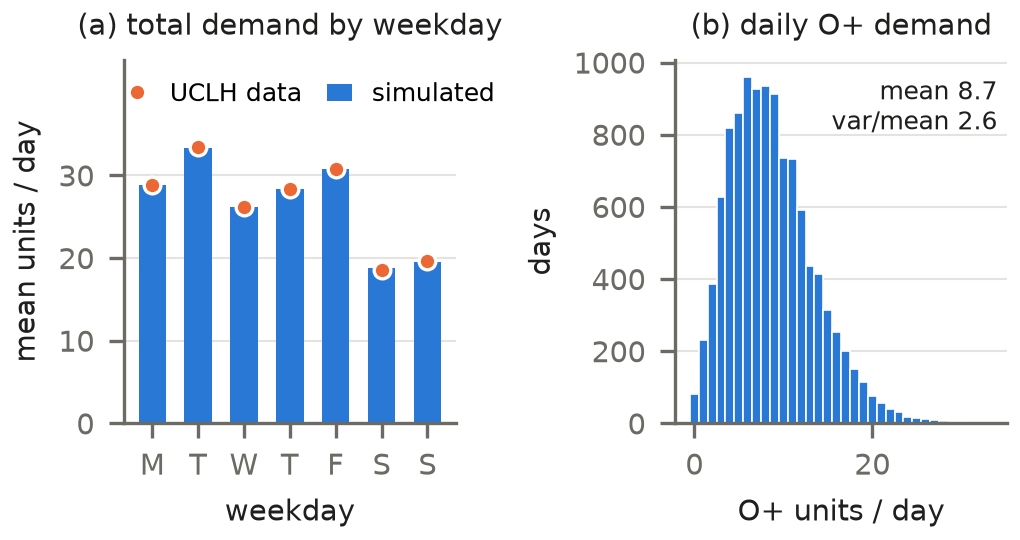
\includegraphics[width=\columnwidth]{../figures/demand_profile.png}
  \caption{Demand calibration over 30 simulated years. (a) Simulated mean total demand per weekday against the UCLH values~\cite{uclh2024platelet}. (b) Daily O+ demand; the pooled variance/mean is above 2.28 because the mean also changes by weekday.}
  \label{fig:demand}
\end{figure}

\textbf{State space $\mathcal{S}$.} For $G$ blood groups the observation contains (i) the stock of each group split by remaining shelf life of 1 to 5 days ($5G$ values), (ii) the units ordered yesterday that arrive tomorrow ($G$), (iii) the last 7 days of demand of each group ($7G$) and (iv) a one-hot encoding of the weekday (7). This gives $13G+7$ features: 111 for the full problem ($G=8$) and 20 for the single-group (O+) version. Each part is divided by a fixed constant (50 for stock, 25 for orders, 40 for demand).

\textbf{Action space $\mathcal{A}$.} The agent orders $q_g \in \{0,\dots,25\}$ units of every group, so $\mathcal{A}$ is MultiDiscrete $26^8$ for the full problem (used with PPO~\cite{schulman2017ppo}) and Discrete 26 for the single group (used with DQN~\cite{mnih2015dqn}).

\textbf{Transition dynamics.} One step is one day. (1) Yesterday's order arrives, and each unit gets a remaining life of 3, 4 or 5 days with probability 0.2, 0.3 and 0.5. (2) Today's order is placed and arrives tomorrow (lead time of one day). (3) Demand is sampled. (4) Each group is served from its own stock, oldest units first (FIFO). (5) Remaining demand is met by compatible donor groups, e.g.\ AB+ can receive from any group and O$-$ only from O$-$; a donor only gives units that its own patients did not need today. (6) Demand still unmet is a shortage (an emergency order). (7) Units with one day of life left expire and all other units age by one day. An episode lasts 365 days.

\textbf{Reward $\mathcal{R}$.} The reward is the negative daily cost, summed over groups:
\begin{equation}
r_t = -0.01 \sum_{g} \left( 10\,s_g + 0.5\,u_g + 3\,e_g + 0.1\,h_g + q_g \right),
\end{equation}
where $s_g$ is shortage, $u_g$ substituted units, $e_g$ expired units, $h_g$ end-of-day stock and $q_g$ units ordered. A shortage costs the most because it directly harms a patient; expiry is the next most costly because the unit was paid for and a donation was wasted. Substitution is cheap but not free, because it uses up rare groups such as O$-$. The small holding cost discourages very large stock, and the factor 0.01 keeps rewards in a range suitable for neural network training.

\textbf{Baselines.} We compare the RL agents with three rules: \emph{random} orders; \emph{mean demand}, which orders the expected demand of the day the order arrives; and \emph{base stock}, which raises stock plus pipeline to $k$ days of mean demand. The level $k$ is chosen by grid search over $1.0,1.25,\dots,5.0$ on 20 tuning seeds that are separate from the evaluation seeds, giving $k=3.5$ (all groups) and $k=3.75$ (O+ only). All environments and baselines are implemented with Gymnasium, and the agents use Stable-Baselines3~\cite{raffin2021sb3}.
